\documentclass{article}
\usepackage[utf8]{inputenc}
\usepackage{amsmath}
\usepackage{tikz}
\usepackage{amssymb}
\usepackage{graphicx}
\usepackage{pgfplots}
\usepackage{parskip}
\usepackage{amsmath}
\usepackage{fullpage}

\title{Vettori}
\author{Paolo Bettelini}
\date{}

\begin{document}

\maketitle
\tableofcontents
\pagebreak

\section{Definitione}

Un vettore è un oggetto geometrico possedente un verso, una direzione ed una intensità. \\
Il vettore non possiede un punto di origine e può essere rappresentato in qualsiasi posizione dello spazio.

Un vettore può essere espresso mediante le sue componenti

\[
    \vec{a} =
    \begin{pmatrix}
        x \\
        y
    \end{pmatrix}
\]

In caso di un vettore n-dimensionale

\[
    \vec{a} =
    \begin{pmatrix}
        \vec{a}_1 \\
        \vec{a}_2 \\
        \vdots \\
        \vec{a}_n
    \end{pmatrix},
    \quad \vec{a} \in \mathbb{R}^n
\]

\section{Addizione vettoriale}

\begin{center}
	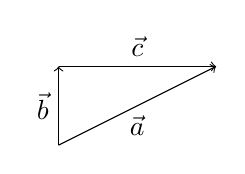
\begin{tikzpicture}]
		\draw [->] (1,1) -- node [below] {\(\vec{a}\)} (3,2);
		\draw [->] (1,1) -- node [left] {\(\vec{b}\)} (1,2);
		\draw [->] (1,2) -- node [above] {\(\vec{c}\)} (3,2);
	\end{tikzpicture}
\end{center}

\[
    \vec{a} + \vec{b} = \vec{c}
\]

\section{Prodotto scalare}

Un vettore \(\vec{a}\) può essere moltiplicato da un valore scalare \(k\)

\[
    k\cdot\vec{a} =
    \begin{pmatrix}
        k\cdot \vec{a}_x \\
        k\cdot \vec{a}_y
    \end{pmatrix},
    \quad k\in\mathbb{R}
\]

\section{Combinazione lineare}

Una combinazione lineare è una somma di due o più vettori, ognuno con un proprio coefficiente

\[
    \vec{c} = a \cdot\vec{a} + b\cdot\vec{b},
    \quad a,b\in \mathbb{R}
\]

\section{Intensità vettore}

Per trovare l'intensità di un vettore possiamo applicare il teorema di pitagora

\[
    ||\vec{a}|| = \sqrt{{a_x}^2 + {a_y}^2}
\]

In caso di un vettore n-dimensionale

\[
    ||\vec{a}|| = \sqrt{{a_1}^2 + {a_1}^2 + \cdots + {a_n}^2},
    \quad \vec{a}\in\mathbb{R}^n
\]

\section{Distanza}

La distanza tra due punti descritti dai vettori \(\vec{a}\) e \(\vec{b}\) è data da

\[
    ||\vec{a}-\vec{b}||
\]

\section{Vettore dati punti}

Possiamo trovare un vettore dati 2 punti \(A\) e \(B\).

\begin{align*}
    &A(A_x; A_y) \\
    &B(B_x; B_y)
\end{align*}

Il vettore dal punto \(A\) al punto \(B\) è dato da

\[
    \begin{pmatrix}
        B_x - A_x \\
        B_y - A_y
    \end{pmatrix}
\]

\section{Vettore unitario}

Il vettore unitario è un vettore di lunghezza \(1\).

\[
    ||\hat{a}|| = 1
\]

Per rendere un vettore unitario è sufficiente dividere le sue componenti per la propria lunghezza.

\[
    \frac{\vec{a}}{||\vec{a}||}=\hat{a}
\]

\(\vec{a}\) non può essere il vettore nullo.

\section{Base}

Una base permette di esprimere qualsiasi vettore nel piano con una combinazione lineare dei vettori della base.

\section{Base ortonormale}

Una base ortonormale è una base con vettori unitari e ortogonali fra di loro.

\[
    \vec{a} = a \cdot \hat{i} + b \cdot \hat{j},
    \quad a,b \in \mathbb{R}
\]

\begin{enumerate}
    \item \(\hat{i}\) è perpendicolare a \(\hat{j}\)
    \item \(\hat{i}\) e \(\hat{j}\) sono unitari
    \item \(\hat{i} \neq a\cdot\hat{j},\quad a\in \mathbb{R}\)  
\end{enumerate}

\section{Vettore posizione}

Il vettore posizione è un vettore che parte dall'origine e va in un punto \(P\).
Questo vettore permette di rappresentare un punto nello spazio cartesiamo con un vettore.

\pagebreak

\end{document}
